\ifx\pfmtname\undefined
\documentclass[a4paper]{article}
\else
\documentclass{article}
\fi
\usepackage{robomech_en}
\usepackage[dvipdfmx]{graphicx}

\begin{document}
\makeatletter
\title{Title: Times New Roman, Bold, 14pt}
{--Subtitle: Times New Roman, Bold, 12pt--}%Change this blank if you don't have a subtitle.
{}%keep this blank
{}%keep this blank

% DO NOT insert [Member / Student Member], if you are an associate academic society member
\author{ \small
\begin{tabular}{ll}
 $\bigcirc$ & Daigoro SHINJUKU, Student Member,  Kikai University, daig\_shinj@kikai.ac.jp\\% $\bigcirc$ represents the presenter
  & Jiro SHIBUYA, Member, Robomec Electric Corporation\\
  & Manabu TOKYO, Member, Nishi University\\
  & [Authors' names, Membership, and Affiliations: Times New Roman, 9pt]
\end{tabular}
}
\makeatother


\abstract{ \small
Papers submitted must be original, and previously unpublished. The responsibility for the contents of published articles rests solely with the authors and not the society. Copyright of the papers published belongs to the JSME (Japan Society of Mechanical Engineers). [Abstract: Times New Roman, 9pt, 100-150words]
}

\date{} % No date
\keywords{Robot, Manipulation,... (no more than five words) [Times New Roman, 9pt]}

\maketitle
\thispagestyle{empty}
\pagestyle{empty}

\small
\section{Introduction [Section Title: 10pt, \protect\\ Bold font, Center-aligned]}%===========================
Main text: Times New Roman, 9pt, and Line intervals: about 4.2 mm.

\subsection{Manuscript requirements [Subsection Title; 9pt, Bold font, Left-aligned]}%-----------
\begin{itemize}
	\item Paper size: A4 (210 $\times$ 297 mm)
	\item Margins: Top and Bottom = 25 mm, Left and Right (title area) = 25 mm, Left and Right (two-column area) = 15 mm, Column separation = 6 mm.
	\item Font settings: Refer to the \reftab{tbl: table1}.
	\item Resolution of figures: High resolution image that are more than 300 dpi.
	\item Captions of figures and tables: “Fig.\# Title of the figure” and “Table \# Title of the table.”
    \item Axis names: Do not use just variables but show specific words and units for representing the axes.
	\item Equations: Describe equations at the center of line and specify equation numbers with a right alignment. In texts, show the equation numbers like “\refeqn{eqn: eq1}.”
	\begin{equation}
		M\ddot{r}_{str1} + F_{frk} = Mg
		\label{eqn: eq1}
	\end{equation}

	\item Unit systems: Use the SI units.
	\item When you refer literature in the texts,  insert the reference number after the words or sentences referred (For example, the study\cite{Shinjuku98}). If the referred word is a subject or an object, do not use the reference number alone but describe like “The study\cite{Shinjuku98} reports ... .”
	\item Prefix $\bigcirc$ to the author's name who make a presentation.
	\item Your manuscript should be converted to a PDF.  Please submit only the PDF. Follow the instruction on the website to submit the manuscript. 
	\item[] 
	\item[*] Note that the file size of the PDF must be less than 2 MB, and the page length is 2--4 pages. 
	\item[*] Do not include the Paper ID, the conference name, and page numbers. 
\end{itemize}

\begin{table}[tb]
 \caption{Type size and typefaces for papers}
 \label{tbl: table1}
 \centering
 \footnotesize
 \begin{tabular}{|p{35mm}|l|l|l|}
  \hline
	Contents	&Fonts \\\hline
	Normal text	&Times New Roman 9pt \\\hline
	Title	&Times New Roman, bold, 14pt \\\hline
	Subtitle	&Times New Roman, bold, 12pt \\\hline
	Authors Names	&Times New Roman 9pt \\\hline
	Abstract and Keywords	&Times New Roman 9pt \\\hline
	Section title		&Times New Roman, bold, 10pt \\\hline
	Subsection title		&Times New Roman, bold, 9pt \\\hline
	Captions of Figures and Tables	 &Times New Roman 9pt \\\hline
	References		&Times New Roman 8pt \\
  \hline
 \end{tabular}
\end{table}

\begin{figure}[tbh]
 \centering
  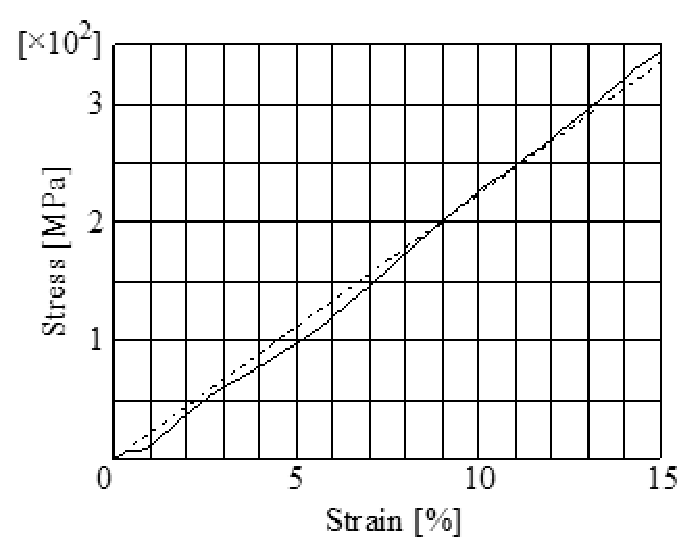
\includegraphics[height=38mm]{fig1.eps}
  \vspace*{-4mm}
  \caption{Tensile stress-strain diagram}
  \label{fig: fig1}
\end{figure}

\footnotesize
\begin{thebibliography}{99}

\bibitem{Shinjuku98}
Daigoro Shinjuku, Jiro Shibuya, and Manabu Tokyo, ``Study on Robotics and Mechatronics,'' {\it Trans. of the JSME. C}, vol. 19, no. 1, pp. 3856--2864, 1998.


\bibitem{Shinjuku99}
Shinjuku, D., Shibuya, J. and Tokyo, M., ``Swing Motion Control of Casting Manipulation,'' {\it IEEE Control Systems}, vol.19-4, pp.56--64, 1999.

\end{thebibliography}

\normalsize
\end{document}
